\documentclass[aspectratio=169]{beamer}

\usepackage[utf8]{inputenc}
\usepackage{default}
\usepackage[spanish]{babel}
\usepackage{amsmath}
\usepackage{amsfonts}
\usepackage{amssymb}
\usepackage{subfig}
% 

\begin{document}


\title{\textbf{Sistema de transmisión segura punto a punto y multipunto en medios compartidos.}}


\author{\small Alfredo Adrián Ortega\\
Instituto Tecnológico de Buenos Aires (ITBA) \\
     aortega@alu.itba.edu.ar\\    }





\frame{\titlepage

\begin{columns}
  \begin{column}{0.99\textwidth}

\begin{figure}[h]
  \centering
    \hspace{0.8cm} \includegraphics[height=0.7cm]{graphs/ITBA_sfondo2.png}
\end{figure}

  \end{column}

  \begin{column}{0.01\textwidth}

  \end{column}
\end{columns}
}

%% TOC

\frame{\frametitle{Contenido}\tableofcontents[hideallsubsections]}




%------------------------------------------------------------
\section{Introducción}
\begin{frame}{Introducción}

%\begin{columns}
%  \begin{column}{0.60\textwidth}

\begin{itemize}
 \item Tema: Privacidad en redes de acceso utilizando CDMA.
 \item Algoritmo criptográficamente seguros.
 \item Velocidades de 5 GBPS o mas.
 \item Subtema: comunicaciones \color{red}acústicas \color{black} privadas.
\end{itemize}

%\end{column}
 % \begin{column}{0.40\textwidth}

  \begin{figure}[!t]
   \centering
   \subfloat[Red óptica]{{\includegraphics[width=0.25 \textwidth]{../graphs/ftth.pdf} }}%
   \qquad
   \subfloat[Red acústica]{{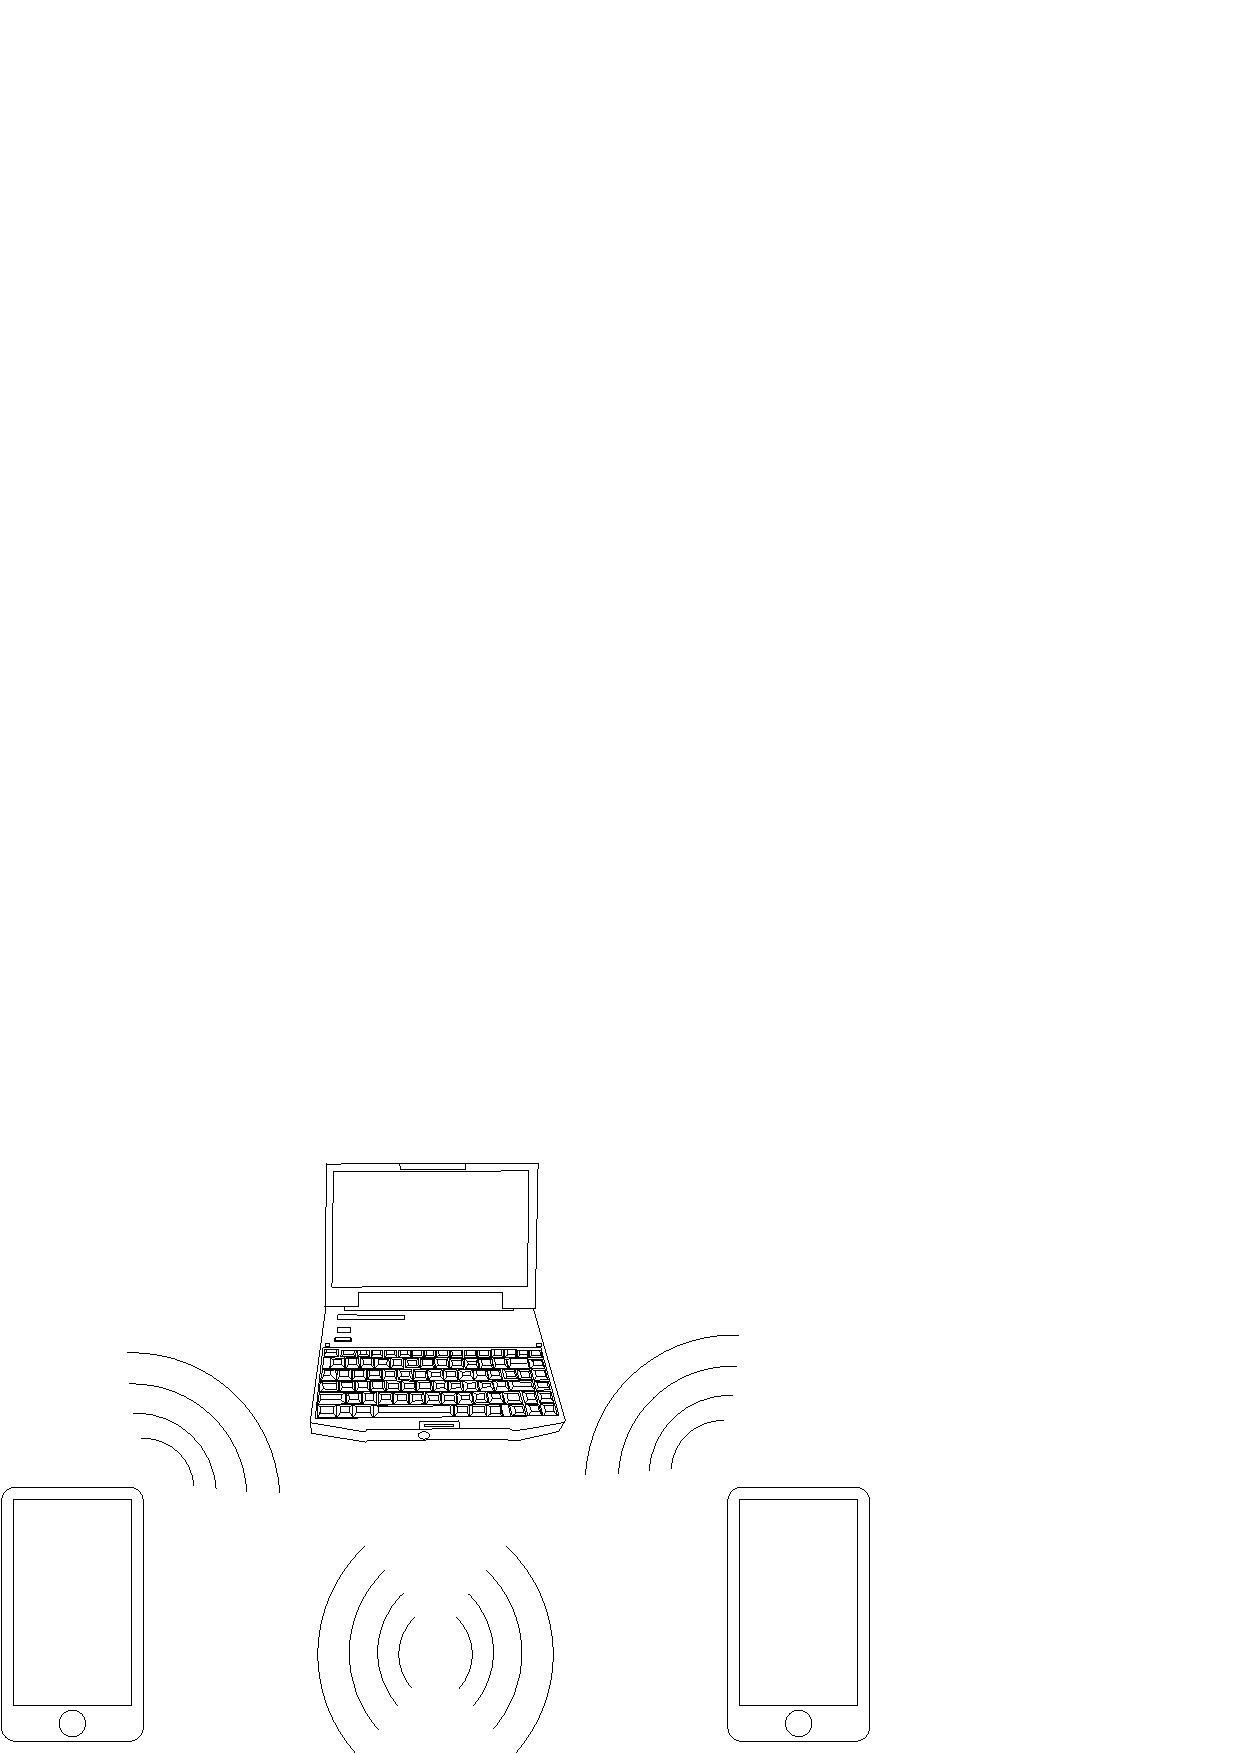
\includegraphics[width=0.25 \textwidth]{../graphs/compucelus.pdf} }}%
   \qquad
  %\caption {Diagramas de ojo de la señal óptica a la salida de la fibra. Se observa una degradación importante de la calidad de la señal al aumentar la tasa de bits.}
  \label{fig:ImgOjo}
\end{figure}

%  \end{column}
%\end{columns}

\end{frame}
%------------------------------------------------------------


\begin{frame}{Problemas a resolver}

\begin{itemize}
 \item Privacidad de datos en una red que utiliza un medio compartido
 \item Protección ante nodos maliciosos
 \item Eliminar toda fuga de información
 \end{itemize}
\end{frame}
%------------------------------------------------------------

\begin{frame}{Solución propuesta}
\begin{columns}
  \begin{column}{0.60\textwidth}

\begin{enumerate}
 \item Utilizar CDMA para la separación en canales
 \item Desarrollar algoritmos criptográficamente seguros para la privacidad
 \end{enumerate}

  \end{column}
  \begin{column}{0.40\textwidth}

 
\begin{figure}[t]
  \centering
  \includegraphics[width=0.55 \textwidth]{../graphs/tdmacdma} 
  \label{fig_tdmacdma}
\end{figure}

  \end{column}
\end{columns}

\end{frame}
%------------------------------------------------------------

\begin{frame}{Desafíos}
\begin{columns}
  \begin{column}{0.60\textwidth}

\begin{enumerate}
 \item Sistema capaz de operar a 5 Gbps+
 \item Evitar protocolos de control que debiliten la criptografía
 \item Aislación completa de canales de comunicación, para evitar ataques del tipo \textit{side channel}.
 \item Bajo costo
 \end{enumerate}

  \end{column}
  \begin{column}{0.40\textwidth}
 
 
 \begin{figure}[!t]
   \centering
   \includegraphics[width=0.80 \textwidth]{../graphs/medicionesPaper/eye71G.png}
   \qquad
   Diagramas de ojo, tasa de $7.5$ Gbps, 20 ns por división.
%  \caption {Diagramas de ojo, tasa de $7.5$ Gbps, 20 ns por división.}
  \label{fig:ImgOjo}
\end{figure}


\end{column}
\end{columns}

\end{frame}

%-------------------------------------------------------------

\section{Estado del Arte}
\frame{\tableofcontents[currentsection,hideallsubsections]}

\frame{\frametitle{Seguridad en las capas de red}
%\framesubtitle{ Capas de red}

\begin{columns}
  \begin{column}{0.40\textwidth}

\begin{figure}[t]
  \centering
    \includegraphics[width=0.80\textwidth]{graphs/layers.pdf}
    \\ Modelo de red OSI simplificado
    \label{ios_process_mem}
\end{figure}

  \end{column}
  \begin{column}{0.65\textwidth}

  \begin{itemize}
      \item SSH
      \item SSL
      \item Kerberos
  \end{itemize}
  \pause\vfill
  {\bf Desventajas:}
	  \begin{itemize}
	  \item Usualmente \alert{mal configurada}
	  \item Directamente \alert{olvidada}
	  \end{itemize}	  

  \end{column}
\end{columns}

}


\frame{\frametitle{Seguridad en las capas de red}
%\framesubtitle{Capa física}

\begin{columns}
  \begin{column}{0.40\textwidth}

\begin{figure}[t]
  \centering
    \includegraphics[width=0.80\textwidth]{graphs/layers.pdf}
    \\ Modelo de red OSI simplificado
    \label{ios_process_mem}
\end{figure}

  \end{column}
  \begin{column}{0.65\textwidth}

  \begin{itemize}

    \item Reflectores de tipo red de Bragg (\textit{Bragg Grating}) \cite{torres2002}
	  \begin{itemize}
	  \item Configuración \alert{fija}
	  \end{itemize}

    \vfill\pause
	  
    \item Sistema propuesto en~\cite{mosso2011all}
	\begin{itemize}
	\item Baja cantidad de canales (\alert{crosstalk})
	\item Espacio de claves \alert{reducido}
     \end{itemize}
     
     \vfill\pause
	  
    \item CDMA \& códigos Walsh \cite{Nadarajah2006}
	  \begin{itemize}
	  \item Espacio de claves \alert{muy reducido} \cite{Shake:05}
	  \end{itemize}
	
      \end{itemize}

  \end{column}
\end{columns}

}


%\frame{\frametitle{Security in the layered network model}


%\begin{itemize}

% \item Aplying Advanced Encryption Standard (AES, see~\cite{Daemen98aesproposal:}) to data, then sent by direct sequence CDMA with a short code% ength~\cite{Wang:10}.
% \begin{itemize}
% \item Altough this method offers privacy and high channel utilisation, it is limited to point-to-point communication. % vb 121122
% \end{itemize}
%\end{itemize}

%}

\section{Sistema propuesto}
\frame{\tableofcontents[currentsection,hideallsubsections]}

\frame{\frametitle{Sistema propuesto}
\vfill
\textbf{Basado en:}
\begin{description}
 \item[Time-hopping CDMA:] El tiempo de transmisión se selecciona mediante un algoritmo generador de números pseudoaleatorios (\alert{PRBS}).
 \item[Filtro de Bloom:] Provee \alert{corrección de errores} asimétrica (en un canal Z)\vfill
 \item[Minimización de peso de Hamming:] \alert{reducción} de símbolos problemáticos en el canal Z\vfill
\end{description}
\vfill
\pause
\textbf{Ventajas:}
  \begin{itemize}
  \item Punto-a-punto y Punto-a-\alert{multipunto}\vfill
  \item \alert{Privacidad}\vfill
  \end{itemize}
\vfill
}

\frame{\frametitle{Sistema propuesto: diseño de alto nivel}
\begin{figure}[t]
\centering
\includegraphics[width=2.5in]{../graphs/hub}
\label{fig_hub}
\end{figure}
}

\frame{\frametitle{Sistema propuesto: diagrama esquemático}
\begin{figure}[t]
\centering
\includegraphics[width=3.5in]{../graphs/Soft-stack3}
\label{fig_comstack}
\end{figure}
}



%-------------------------------------------------------------

\section{Metodología}
\frame{\tableofcontents[currentsection,hideallsubsections]}

%------------------------------------------------------------
\subsection{Canal Z}
\begin{frame}{Canal Z}
\begin{figure}[t]
  \centering
    \includegraphics[width=5cm]{../graphs/zchannel.pdf}
    
    Diagrama de probabilidad del canal binario asimétrico o canal Z.
\end{figure}
\end{frame}

%------------------------------------------------------------
\subsection{Time hopping}
\begin{frame}{Selección de casillero aleatoria: \textit{time hopping}}
\begin{figure}[t]
  \centering
    \includegraphics[width=8cm]{graphs/slide2.pdf}
    \\ \huge No hay colisión
\end{figure}
\end{frame}
%------------------------------------------------------------
\begin{frame}{Selección de casillero aleatoria: \textit{time hopping}}
\begin{figure}[t]
  \centering
    \includegraphics[width=8cm]{graphs/slide3.pdf}
    \\ \huge Colisión $\Rightarrow$ \textcolor{blue}{Resultado OK}
\end{figure}
\end{frame}
%------------------------------------------------------------
\begin{frame}{Selección de casillero aleatoria: \textit{time hopping}}
\begin{figure}[t]
  \centering
    \includegraphics[width=8cm]{graphs/slide4.pdf}
    \\ \huge Colisión $\Rightarrow$ \textcolor{red}{Error}
\end{figure}
\end{frame}
%------------------------------------------------------------
\subsection{Filtro de Bloom}
\begin{frame}{CDMA + Filtro de Bloom (K=3)}
\begin{figure}[t]
  \centering
    \includegraphics[width=8cm]{graphs/z_bloom1.pdf}
    \\ \huge Inserta el bit '1' en la trama
\end{figure}
\end{frame}
%------------------------------------------------------------
\begin{frame}{CDMA + Bloom filter (K=3)}
\begin{figure}[t]
  \centering
    \includegraphics[width=8cm]{graphs/z_bloom2.pdf}
    \\ \huge Inserta el bit '0' en la trama
\end{figure}
\end{frame}
%------------------------------------------------------------
\begin{frame}{CDMA + Bloom filter (K=3)}
\begin{figure}[t]
  \centering
    \includegraphics[width=8cm]{graphs/z_bloom3.pdf}
    \\ \huge Inserta el bit '1' en la trama $\Rightarrow$ \textcolor{red}{Error}
\end{figure}
\end{frame}


%------------------------------------------------------------
\subsection{K óptimo}
\begin{frame}{K óptimo}

\begin{figure}[!t]
  \centering
    \includegraphics[width=3in]{../graphs/Kcalc}
    
    Estimación de BER vs. tasa de repetición de filtro de Bloom K.
    \label{BERvsK}
\end{figure}

\begin{equation}
\text{BER} \approx \frac{n}{2} m_0 z_{\bar{R},\bar{S}} \approx \frac{n}{2} m_0 \left(1-e^{-W_1/M}\right)^K.
\end{equation}
\end{frame}

%------------------------------------------------------------

\subsection{Minimización del peso de Hamming}

\frame{\frametitle{Minimización del peso de Hamming}
\framesubtitle{Símbolo de 3-bits, Peso de Hamming=2, expansión a 5 bits}
\begin{center}
\begin{tabular}{c c c}

Dato & Entrada, HW=variable & Expansión HW=2\\
\hline\hline
0 & 000 & 00011\\
1 & 001 & 00110\\
2 & 010 & 00101\\
3 & 011 & 01100\\
4 & 100 & 01010\\
5 & 101 & 01001\\
6 & 110 & 10001\\
7 & \alert{111} & \alert{1}00\alert{1}0\\
\end{tabular}
\end{center}

%Example Hamming minimisation table for a 3-bit input symbol with variable hamming weight,
%output is a 5-bit expanded symbol with fixed Hamming weight HW=2
}


%-------------------------------------------------------------

\section{Implementación y mediciones}
\frame{\tableofcontents[currentsection,hideallsubsections]}

\subsection{Fibra óptica}

\begin{frame}{Implementación: Fibra óptica}

\begin{figure}[t]
  \centering
      \subfloat[Distribución via acoplador tipo estrella 1]{{\includegraphics[width=0.4 \textwidth]{graphs/StarCoupler} }}%
    \qquad
    \subfloat[Distribución via EDFA]{{\includegraphics[width=0.4 \textwidth]{graphs/EDFA} }}%
    
    Diseño de red propuesto para la capa óptica
    \label{arch:fig1}
\end{figure}

\end{frame}

%-------------------------------------------------------------
\begin{frame}{Implementación: Fibra Óptica}

\framesubtitle{Placas de desarrollo Xilinx ML507}
  \centering
  \includegraphics[width=0.7\textwidth]{graphs/fpga.jpg} 

\end{frame}

%-------------------------------------------------------------
\begin{frame}{Implementación: Fibra óptica}

\begin{figure}[t]
  \centering
    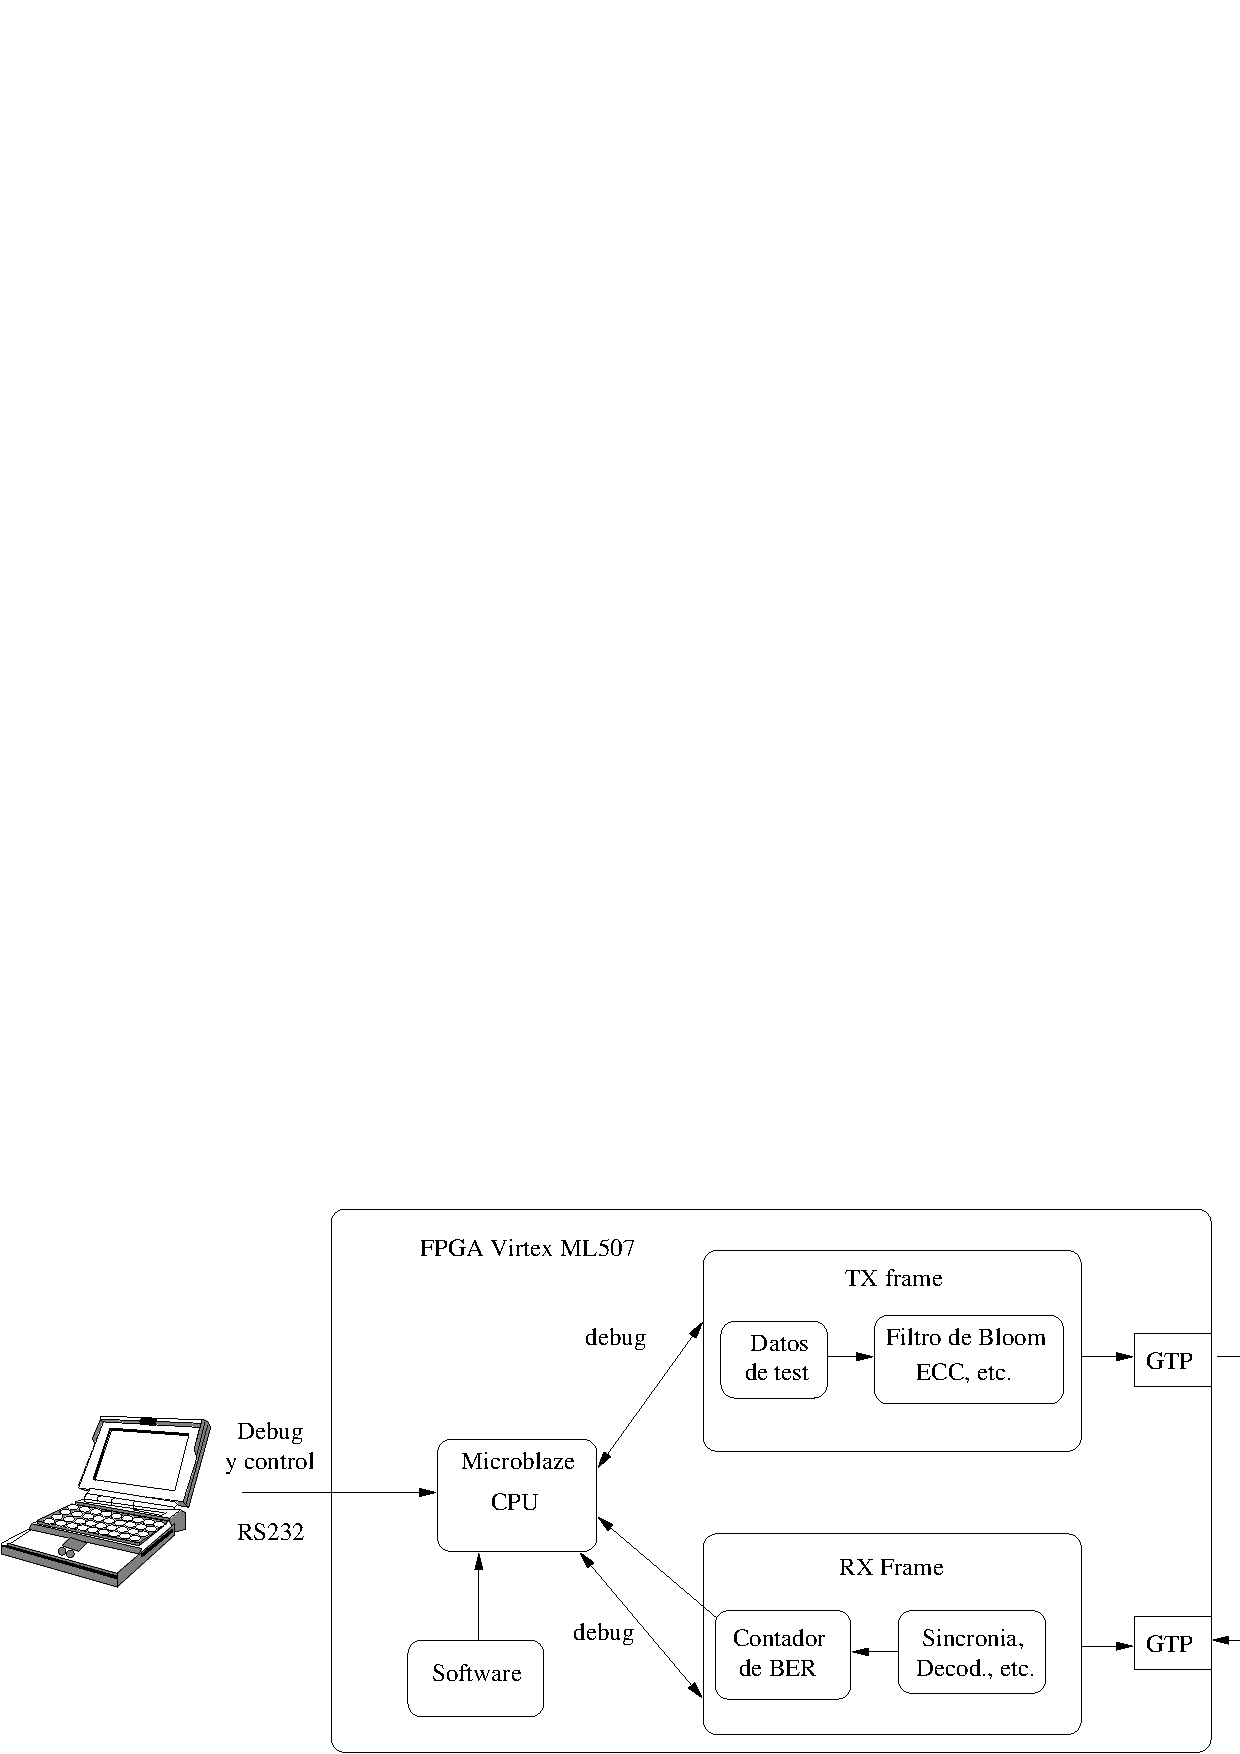
\includegraphics[width=3.3in]{../graphs/fpgadesign.pdf}
     
     Diseño lógico de alto nivel sobre FPGA
\label{fig:fpgadesign}
\end{figure}

\end{frame}

%-------------------------------------------------------------
\begin{frame}{Implementación: Fibra óptica, FPGA}

\begin{figure}[t]
  \centering
    \includegraphics[width=3.5in]{../graphs/diagramaXilinx.png}
\label{fig:fpgahard}
\end{figure}

\end{frame}

%-------------------------------------------------------------
\begin{frame}{Implementación: Fibra óptica, Resultados (Simulaciones)}

\begin{figure}[!t]
  \centering
    \includegraphics[width=4in]{../graphs/BERvsChannelES2}
    
    Desempeño del sistema con respecto a la expansión de símbolo. Simulación numérica de un enlace de 10 Gbps con 128 clientes, M=4096 y K=9.
    \label{BERvsExpansion}
\end{figure}

\end{frame}


%-------------------------------------------------------------
\begin{frame}{Implementación: Efectos de señal desbalanceada}


\begin{figure}[!t]
   \centering
   \subfloat[Señal con 256 bits en uno por trama (8B/10B), 400 ps por bit]{{\includegraphics[width=0.45 \textwidth]{../graphs/expansion1.jpg} }}%
   \qquad
   \subfloat[Señal con 48 bits en uno por trama, 1100 ps por bit]{{\includegraphics[width=0.45 \textwidth]{../graphs/expansion2.jpg} }}%
   \qquad
   
  \vspace{0.2cm}
  Señal de potencia óptica de un Láser SPF+ de 1330 nm, tasa nominal es de 2.5 Gbps.
  \label{fig:ImgExpansion}
\end{figure}
\end{frame}

%------------------------------------------------------------
\subsection{Medio acústico}

\begin{frame}{Medio acústico: introducción}

\begin{figure}[t]
  \centering  
    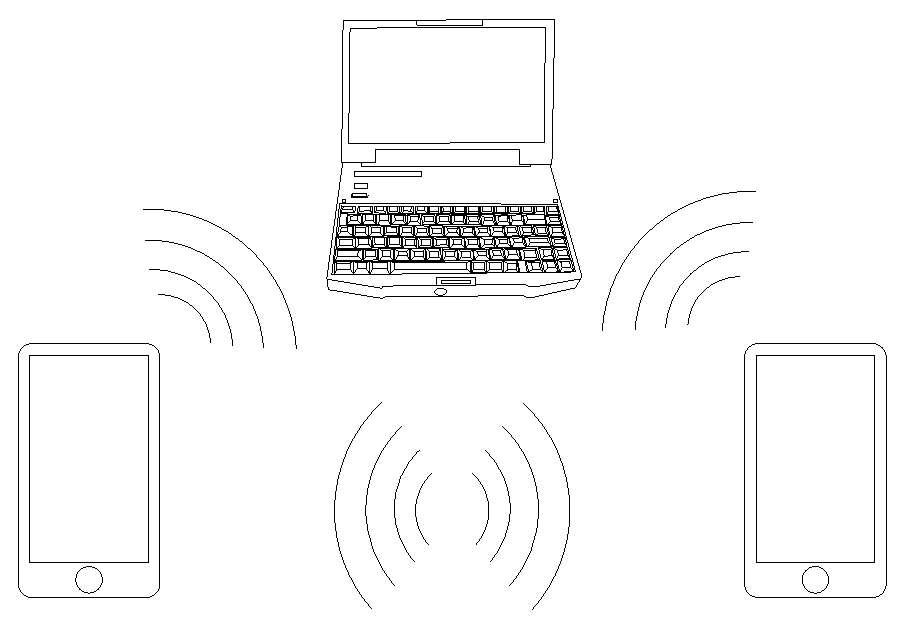
\includegraphics[width=6cm]{graphs/compucelus}
    \vspace{0.5cm}
    \\ Esquema de transmisión acústica
    \label{ios_process_mem}
\end{figure}

\begin{itemize}
 \item Originalmente plataforma de testing del medio óptico
 \item Fácil de depurar e implementar (100\% software)
 \item Equivalente a un módem por software
\end{itemize}

\end{frame}
%------------------------------------------------------------
\begin{frame}{Medio acústico: modulación}

\begin{columns}
  \begin{column}{0.40\textwidth}

  \begin{figure}[t]
  \centering
    \includegraphics[width=5cm]{graphs/modulated.pdf}
    
    Modulación OOK.
    \label{arch:sync}
\end{figure}

  \end{column}
  \begin{column}{0.50\textwidth}
\begin{figure}[th]
  \begin{center}
    \vspace{0.7cm}
    \includegraphics[width=3cm]{../graphs/zchannel}
    
    Diagrama de probabilidad: canal Z.
  \end{center}
  \label{fig:Gal}
\end{figure}

  \end{column}
\end{columns}
\vspace{0.2cm}

\begin{itemize}
 \item Interferencia de OOK se aproxima a la de un canal Z.
 \item Baja densidad espectral (0.2 bits/s/Hz)
\end{itemize}

\end{frame}
%------------------------------------------------------------

\begin{frame}{Medio acústico: sincronización}

\begin{figure}[t]
  \centering  
    \includegraphics[width=6cm]{graphs/acusync}
    \\ Sincronización de bit/nivel de decisión
    \label{ios_process_mem}
\end{figure}

\end{frame}
%------------------------------------------------------------

\begin{frame}{Medio acústico: características y espectro}

\begin{figure}[t]
  \centering  
    \includegraphics[width=10cm]{graphs/spectrum.png}
    \\ Espectro de señal modulada
    \label{ios_process_mem}
\end{figure}

\begin{itemize}
 \item Portadora a 12 Khz, modem funcionando a 1 Kbps en total
 \item Velocidades de 350 bps (2 usuarios) a 70 bps (10 usuarios)
 \item Dispositivos móviles: buen desempeño parlante/micrófono de 100 a 15 Khz
\end{itemize}

\end{frame}

%------------------------------------------------------------
\begin{frame}{Medio acústico: resultados (mediciones)}
  
  \begin{figure}[t]
  \centering  
    \includegraphics[width=8cm]{graphs/medidas_clientes_JIS-fig6}
    \\ BER $vs.$ número de clientes
    \label{ios_process_mem}
\end{figure}

\end{frame}

%------------------------------------------------------------
\begin{frame}{Medio acústico: resultados (mediciones)}
  
\begin{figure}[t]
  \centering  
    \includegraphics[width=8cm]{graphs/mediciones-distancia-fig7}
    \\ BER $vs.$ distancia
    \label{ios_process_mem}
\end{figure}

\end{frame}


%-------------------------------------------------------------

\section{Conclusión}
\frame{\tableofcontents[currentsection,hideallsubsections]}

\frame{\frametitle{Conclusiónes:}
\begin{itemize}
\item Se propuso una arquitectura de red de tipo \alert{time-hopping CDMA}:\pause\vfill
  \begin{itemize}
  \item Punto-a-Punto, y Punto-a-\alert{Multipunto}.\pause\vfill
  \item \alert{Red Privada} y criptográficamente segura.\pause\vfill
  \item Utilizando Filtros de \alert{Bloom} y minimización de peso de \alert{Hamming}.\pause\vfill
  \item {\bf 29\% de utilización del canal.} \vfill
  \end{itemize}
\end{itemize}
}

%-------------------------------------------------------------

\begin{frame}{Contribuciones:}
%\small
\textbf{Altas velocidades de transferencia en fibra óptica utilizando FPGAs de bajo costo. } \textit{A. A. Ortega, V. A. Bettachini, D.F. Grosz, J. I. Alvarez-Hamelin - Congreso de Microelectrónica Aplicada 2010 BsAs}

\

\textbf{ Point-to-point and Point-to-multipoint CDMA Access Network with Enhanced Security} \textit{ A. A. Ortega, V. A. Bettachini, J. I. Alvarez-Hamelin,  D.F. Grosz, Advanced Photonics 2011 Congress - Access Networks and In-house CommunicationsAccess Networks and In-house Communications, OSA Technical Digest, Optical Society of America}

\

\textbf{Hamming-weight minimisation coding for CDMA optical access networks with enhanced security} \textit{ A. A. Ortega, V. A. Bettachini, J. I. Alvarez-Hamelin, D.F. Grosz, Future Generation Communication Technology (FGCT), 2012}


\end{frame}

\begin{frame}{Contribuciones:}
%\small
\textbf{Encrypted CDMA Audio Network.} \textit{ A. A. Ortega, V. A. Bettachini, P. I. Fierens, y J. I. Alvarez-Hamelin -  Journal of Information Security - 2014}

\

\textbf{Patente: DISPOSITIVO Y MÉTODO PARA TRANSMISIÓN SEGURA DE DATOS SOBRE CANALES Z MEDIANTE CDMA (AR084155B1)}\textit{José Ignacio ALVAREZ HAMELIN, Victor Alexis BETTACHINI, and Alfredo ORTEGA. PCT, 12 2012. (Asignada)}

\

\textbf{Patente: Device and Method for the Secure Transmission of Data over Z-Channels Using CDMA (P11104EPPC)}\textit{José Ignacio ALVAREZ HAMELIN, Victor Alexis BETTACHINI, and Alfredo ORTEGA. EPO, Julio 2014. (En trámite)}

\
\end{frame}

%-------------------------------------------------------------

\footnotesize

\begin{thebibliography}{7}


\providecommand{\natexlab}[1]{#1}
\providecommand{\url}[1]{\texttt{#1}}
\expandafter\ifx\csname urlstyle\endcsname\relax
  \providecommand{\doi}[1]{doi: #1}\else
  \providecommand{\doi}{doi: \begingroup \urlstyle{rm}\Url}\fi

\bibitem[Daemen et~al.(1998)]{Daemen98aesproposal:}
 J.~Daemen and V.~Rijmen.
\newblock Aes proposal: Rijndael, 1998.

\bibitem[Mosso et~al.(2011)]{mosso2011all}
F.~Mosso, J.~Barrera, M.~Tebaldi, N.~Bolognini, and R.~Torroba.
\newblock All-optical encrypted movie.
\newblock \emph{Opt. Express}, 19\penalty0 (6):\penalty0 5706--5712, 2011.

\bibitem[Nadarajah et~al.(2006)]{Nadarajah2006}
N.~Nadarajah, E.~Wong, and a.~Nirmalathas.
\newblock {Implementation of multiple secure virtual private networks over
  passive optical networks using electronic CDMA}.
\newblock \emph{IEEE Photonics Technology Letters}, 18\penalty0 (3):\penalty0
  484--486, Feb. 2006.
\newblock ISSN 1041-1135.
\newblock \doi{10.1109/LPT.2005.863637}.
\newblock URL
  \url{http://ieeexplore.ieee.org/lpdocs/epic03/wrapper.htm?arnumber=1576846}.

\bibitem[Ortega et~al.(2011)]{ortega11}
A.~A. Ortega, V.~A. Bettachini, J.~I. Alvarez-Hamelin, and D.~F. Grosz.
\newblock Point-to-point and point-to-multipoint cdma access network with
  enhanced security.
\newblock In \emph{Access Networks and In-house Communications, OSA Technical
  Digest (CD), paper ATuB6}, Toronto, Canada, June 2011.

\bibitem[Shake(2005)]{Shake:05}
T.~Shake.
\newblock Security performance of optical cdma against eavesdropping.
\newblock \emph{IEEE Journal of Lightwave Technology}, 23:\penalty0 655--670,
  Feb. 2005.

\bibitem[Torres et~al.(2002)]{torres2002}
P.~Torres, L.~Valente, and M.~Carvalho.
\newblock Security system for optical communication signals with fiber bragg
  gratings.
\newblock 50:\penalty0 13--16, Jan. 2002.

\bibitem[Wang et~al.(2010)]{Wang:10}
Z.~Wang, L.~Xu, J.~Chang, T.~Wang, and P.~R. Prucnal.
\newblock Secure optical transmission in a point-to-point link with encrypted
  cdma codes.
\newblock \emph{IEEE Photonics Technology Letters}, 22\penalty0 (19):\penalty0
  1410 --1412, oct. 2010.
\newblock ISSN 1041-1135.
\newblock \doi{10.1109/LPT.2010.2061223}.

\end{thebibliography}


\end{document}


